\section{Connecting Components} \label{sc:connecting_components}
The components have been defined in the previous sections and their connections and desired interactions will be described and depicted in this section.
\par
The controllers in the function component are dependent on the data classes in the model component. These dependencies have been converted to an aggregation (see \autoref{fig:FinalComponentDesign}), as each controller is in control of non, one, or multiple data classes. This give more coupling, but as controllers need to know exactly what they control, this coupling has been seen as a necessity.
\par
The connection between the controller classes and the \textit{Repository} strategy is a call (see \autoref{fig:FinalComponentDesign}). This is because the controllers simply call the repositories with an instance of the associated data class, in order to communicate with the database.
\par
The user interface component has a connection to the \textit{Session} class in the function component to ensure that the user can only access the functions they need. The connection exists as a call, because the relation's only purpose is to ensure that the user's information is available to the system.
\par
The user interface component also has a connection to the controllers, as the user needs the ability to call functions in the controllers. The connection exists as a call, because the relation's only purpose is to ensure that the users can interact with the data classes.
\par
% The user interface component is also connected with a call relation to the \textit{ExportHandler} class, as the user, if they have admin access, simply calls the function within the \textit{ExportHandler} to export a list of assets.
% \par
% The \textit{FieldController} contains the functionality to add fields to objects that allow it. The user, if they have admin access, should have access to this functionality and therefore, the user interface has a call relation to the \textit{FieldController} in the function component.
% \par
The repository strategy has a connection to the database, to store the different models. This is simply a call relation, as the repositories make calls to the database.
\par
The decisions reasoned above have resulted in the following component diagram (see \autoref{fig:FinalComponentDesign}). The controllers have been grouped in the packaged \textit{Controllers} and data classes from the model component have been grouped in the package labeled \textit{Data classes}. The remaining classes, not present in the diagram, have been removed in order to simplify the diagram and because they have no dependencies on other components.
\par
With the component design constructed and illustrated, the UI can be designed based on this.

\begin{figure}[H]
    \centering
    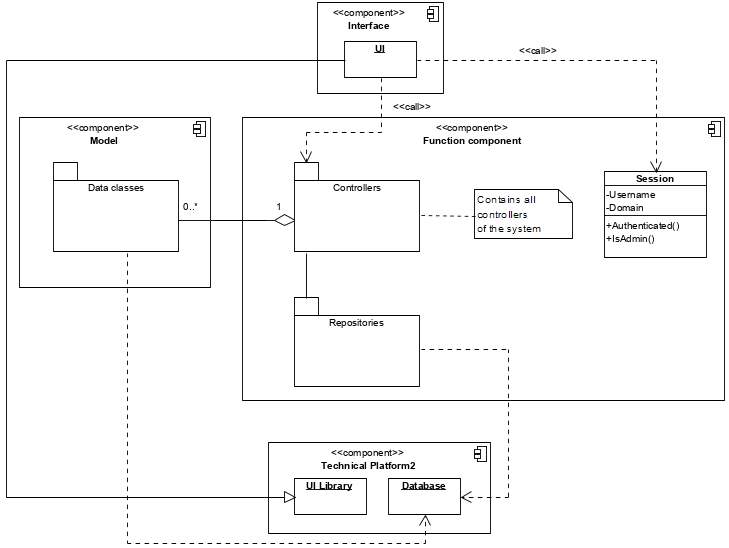
\includegraphics[width=1.3\textwidth,angle=90,origin=c]{figures/ComponentDiagrams/ConnectionOfComponents.png}
    \caption{Illustration of the component design of the system. Only the core classes have been added to the diagram for simplicity.}
    \label{fig:FinalComponentDesign}
\end{figure}